\begin{figure}[!h]
  \centerline{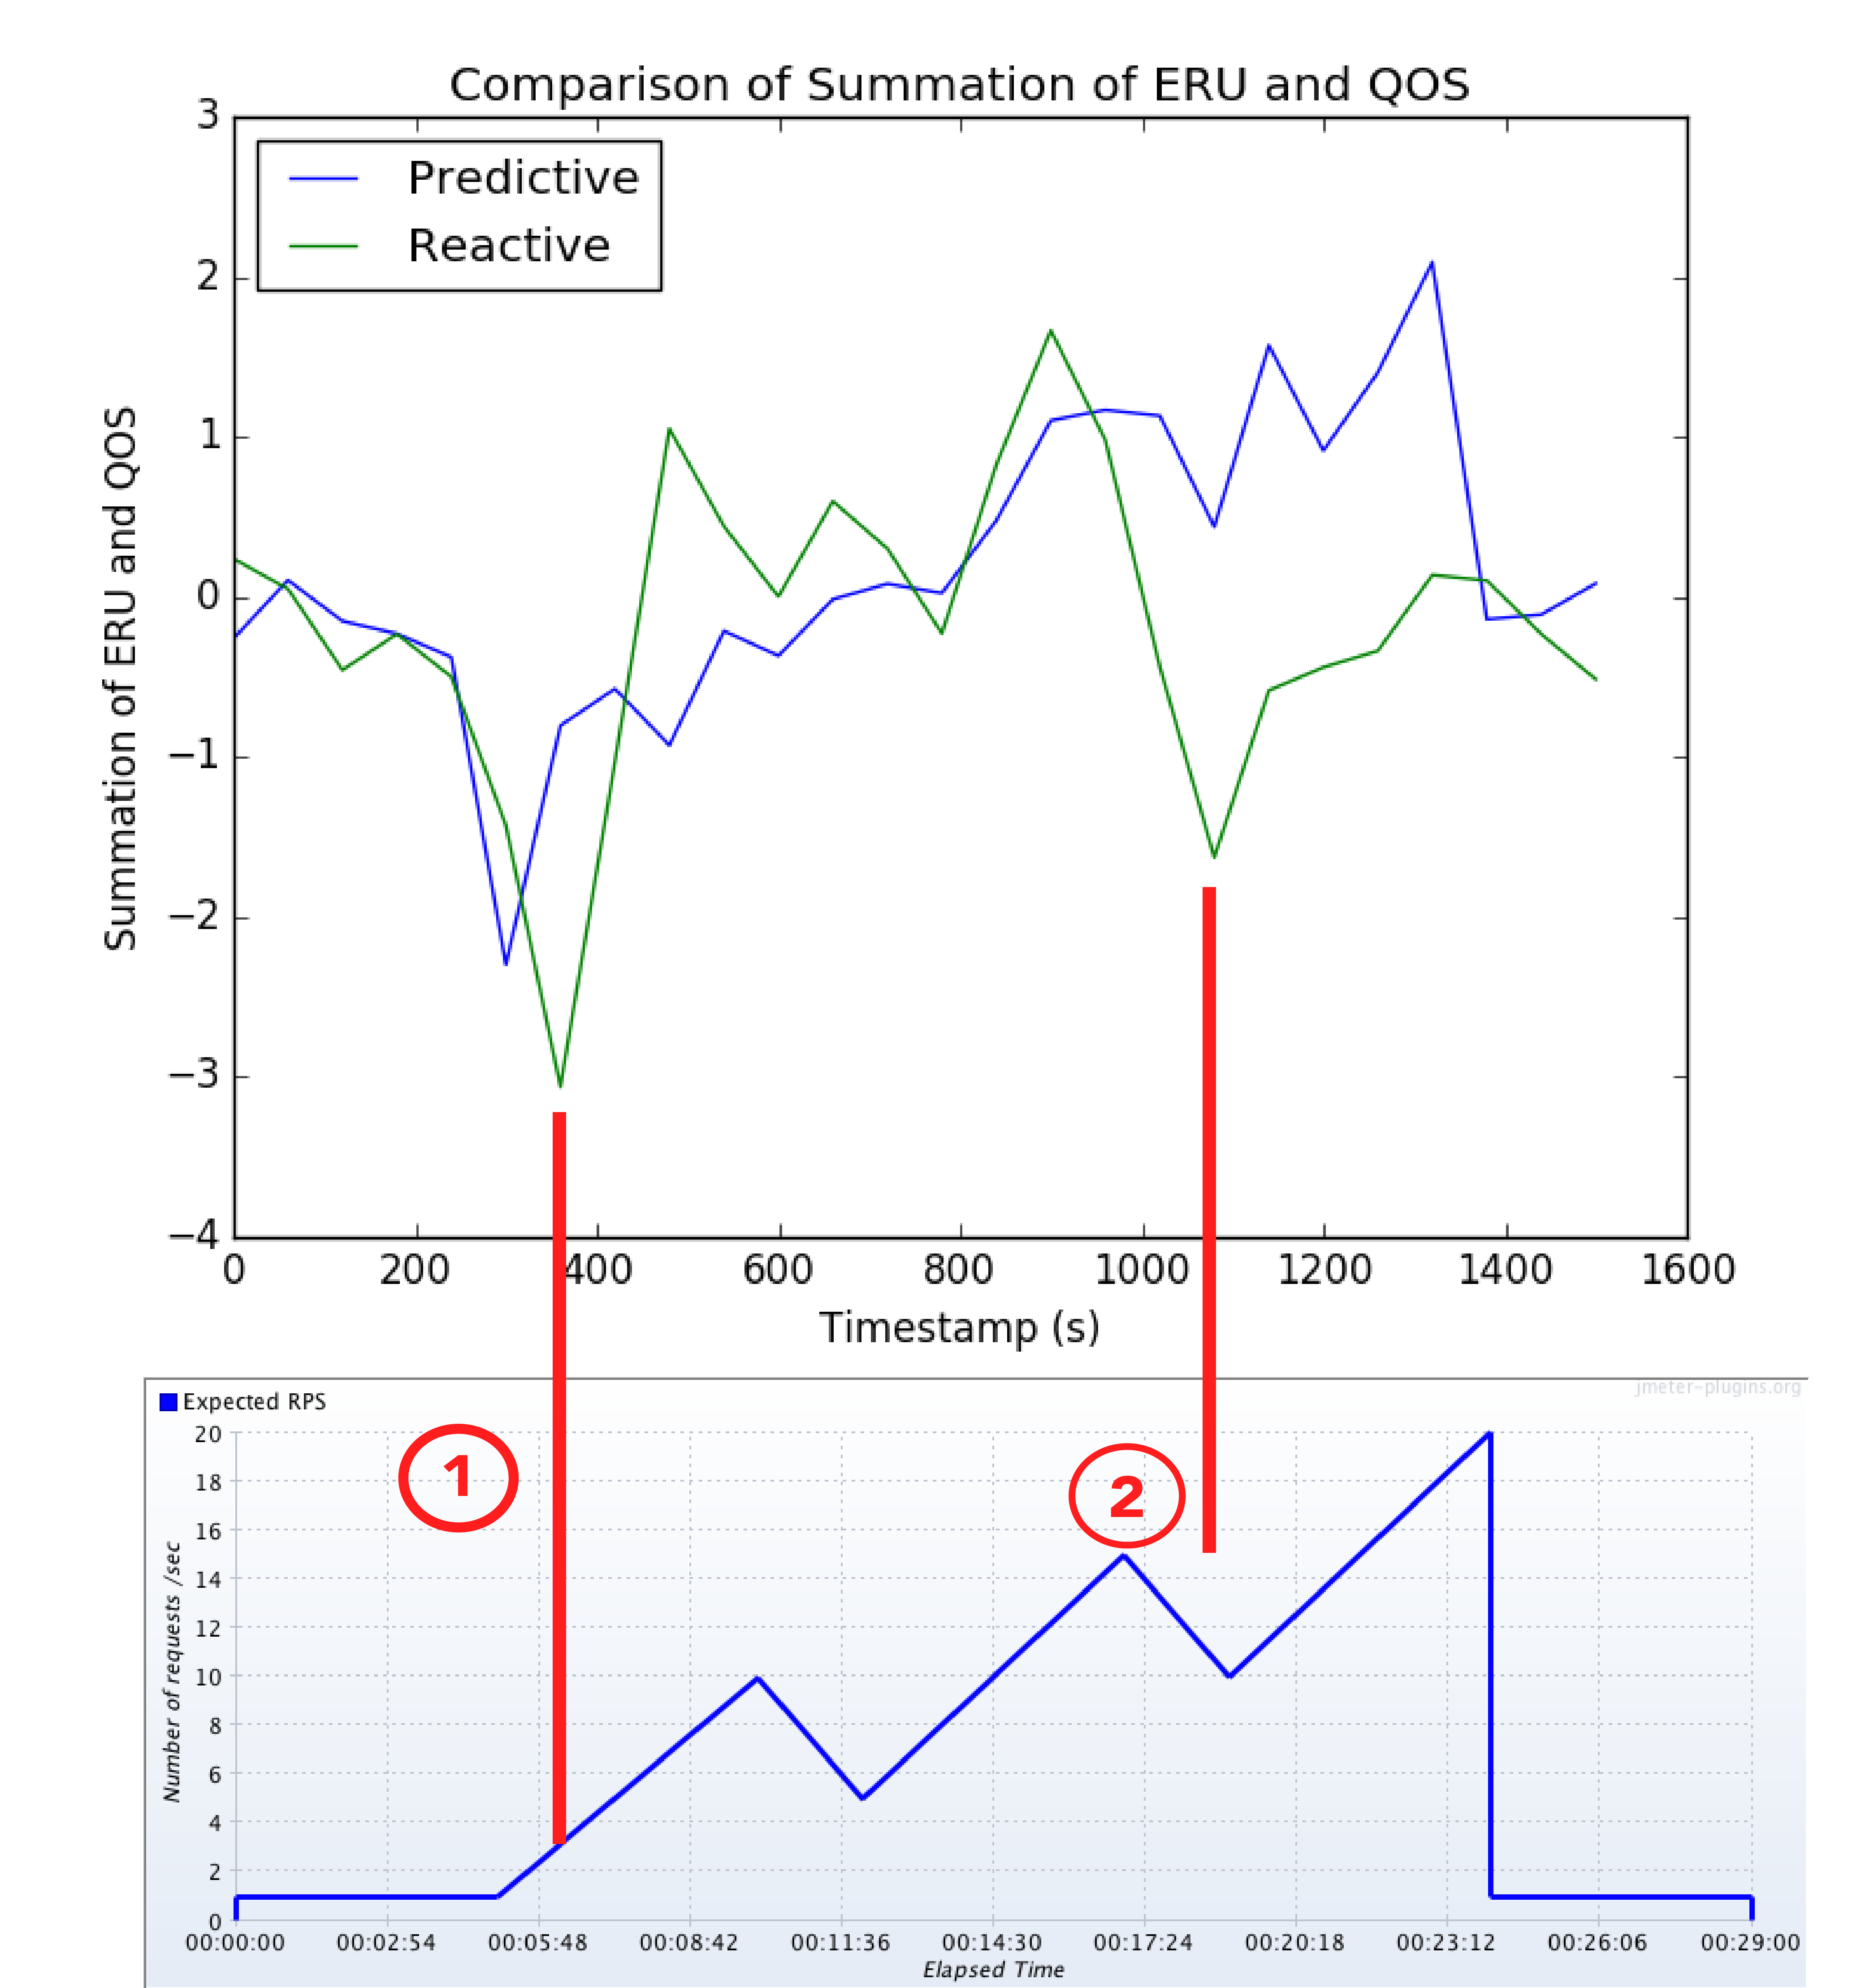
\includegraphics[scale=.70]{jagged-edge-labelled.png}}
  \caption{A comparison of the summation of ERU and QoS for
    predictive and reactive auto-scaling for 135s, jagged-edge.}
  \label{fig:135s-jagged-edge-labelled}
\end{figure}


Figure \ref{fig:135s-jagged-edge-labelled} contains a graph
showing predictive and reactive auto-scaling's different
summations of efficient resource utilization and quality of service over the
course of the \textit{jagged-edge} trial.
The traffic pattern super imposed below reflects the load
placed on the sample application, indicating the effect of the traffic pattern
on the summation of ERU and QoS. Again, we highlight significant times, labelled
$1$ and $2$ for which
predictive auto-scaling has a higher summation of ERU and QoS, and as such is
outperforming reactive auto-scaling. The decrease in the summation of ERU and
QoS for reactive auto-scaling, labelled with the $2$ on the graph, again
reflects the advantages of predictive auto-scaling's ability to understand the
general linear pattern and not drastically under-provision as the result of
temporary downturns.

\begin{table}[htbp]
  \centering
  \caption{Difference in Predictive and Reactive Auto-scaling for 135s,
  jagged-edge.}
  \label{tab:135s-jagged-edge}
\begin{tabular}{l c}\hline\hline
    \multicolumn{1}{c}{\textbf{Measure}} & \textbf{Value} \\ \hline
     p-value & 0.374 \\
     z-score & 0.320 \\
     std\_dev & 1.062 \\
     mean & 0.340
  \end{tabular}
\end{table}

Similarly, while Figure \ref{fig:135s-jagged-edge-labelled} shows the benefits of predictive
auto-scaling on the \textit{jagged-edge} traffic pattern, Table
\ref{tab:135s-jagged-edge} shows that we are unfortunately not able to claim
statistical significance with respect to these results.
